\documentclass[12pt]{article}
\usepackage{graphicx}
\usepackage[none]{hyphenat}
\usepackage{graphicx}
\usepackage{listings}
\usepackage[english]{babel}
\usepackage{graphicx}
\usepackage{caption} 
\usepackage{booktabs}
\usepackage{array}
\usepackage{amsmath}   % for having text in math mode
\usepackage{amssymb} % for \because
\usepackage{extarrows} % for Row operations arrows
\usepackage{listings}
\lstset{
  frame=single,
  breaklines=true
}
\usepackage{hyperref}
  
%Following 2 lines were added to remove the blank page at the beginning
\usepackage{atbegshi}% http://ctan.org/pkg/atbegshi
\AtBeginDocument{\AtBeginShipoutNext{\AtBeginShipoutDiscard}}
\usepackage{gensymb}


%New macro definitions
\newcommand{\mydet}[1]{\ensuremath{\begin{vmatrix}#1\end{vmatrix}}}
\providecommand{\brak}[1]{\ensuremath{\left(#1\right)}}
\providecommand{\sbrak}[1]{\ensuremath{{}\left[#1\right]}}
\providecommand{\norm}[1]{\left\lVert#1\right\rVert}
\providecommand{\cbrak}[1]{\ensuremath{\left\{#1\right\}}}
\providecommand{\abs}[1]{\left\vert#1\right\vert}
\newcommand{\solution}{\noindent \textbf{Solution: }}
\newcommand{\myvec}[1]{\ensuremath{\begin{pmatrix}#1\end{pmatrix}}}
\let\vec\mathbf


\begin{document}

\begin{center}
\title{\textbf{Gradient Descent}}
\date{\vspace{-5ex}} %Not to print date automatically
\maketitle
\end{center}
\setcounter{page}{1}

\section{11$^{th}$ Maths - Chapter 10}
This is Problem-3.1 from Exercise 10.3 
\begin{enumerate}
\item Reduce $x-\sqrt{3}y+8=0$ into normal form. Find its perpendicular distance from the origin and angle between perpendicular and the positive x-axis. 

\solution 
Equation for a line  can be represented in parametric form as
\begin{align}
	\label{eq:Eq2}
	\vec{x} = \vec{A}+\lambda\vec{m}
\end{align}
We choose  
\begin{align}
	\vec{A} &= \myvec{-8 \\ 0}\\
	\vec{O} &= \myvec{ 0 \\ 0} \\
	\vec{m} &= \myvec{1 \\ \frac{1}{\sqrt{3}}} \\
	\text{ yielding }\label{eq:Eq6}
	f\brak{\lambda} &= \frac{4}{3}\lambda^2-16\lambda+64 \\ 
	f^\prime\brak{\lambda} &= \frac{8}{3}\lambda - 16
\end{align}
Computing $\lambda_{min}$ using Gradient Descent method:
\begin{align}
	\lambda_{n+1} &= \lambda_n - \alpha f^\prime\brak{\lambda_n}\\
	\label{eq:grad_des}
	\lambda_{n+1} &= \lambda_n\brak{1-\frac{8}{3}\alpha} + 16\alpha
\end{align}
Taking the one-sided $Z$-transform on both sides of \eqref{eq:grad_des},
\begin{align}
            \label{eq:Z-trans-eqn}
	    z\Lambda\brak{z} &= \brak{1-\frac{8}{3}\alpha}\Lambda\brak{z} + \frac{16\alpha}{1-z^{-1}} \\
	    \Lambda\brak{z} &= \frac{16\alpha z^{-1}}{\brak{1-z^{-1}}\brak{1-\brak{1-\frac{8}{8}\alpha}z^{-1}}} \\
	    &= 6\brak{ \frac{1}{1-z^{-1}} - \frac{1}{1-\brak{1-\frac{8}{3}\alpha}z^{-1}}} \\
            \label{eq:lambda-z-trans}
	    &= 6\sum_{k=0}^{\infty}\brak{1-\brak{1-\frac{8}{3}\alpha}^k}z^{-k}
\end{align}
From \eqref{eq:lambda-z-trans}, the ROC is
\begin{align}
	\abs{z} &> \max\cbrak{1,\abs{1-\frac{8}{3}\alpha}} \\
	\implies -1 & < \abs{1-\frac{8}{3}\alpha} < 1 \\
        \label{eq:alpha-constr}
        \implies 0 &< \alpha < \frac{3}{4}
\end{align}
Thus, if $\alpha$ satisfies \eqref{eq:alpha-constr}, then from \eqref{eq:lambda-z-trans}, 
\begin{align}
	\label{eq:conv}
        \lim_{n\to\infty}\lambda_n &= 6 
    \end{align}
Choosing
\begin{enumerate}
 \item $\alpha$ = 0.001
 \item precision = 0.0000001
 \item n = 10000000 
 \item $\lambda_0$ = -5 
\end{enumerate}
\begin{align}
	\lambda_{min} &= 6 
\end{align}
Substituting the values of $\vec{A}$, $\vec{m}$ and $\lambda_{min}$ in equation \eqref{eq:Eq2} 
\begin{align}
	\vec{x}_{min} &= \vec{P} = \myvec{-8 \\ 0}+6\myvec{1 \\ \frac{1}{\sqrt{3}}}  \\
	&= \myvec{-8 \\ 0}+\myvec{6 \\ \frac{6}{\sqrt{3}}} \\
	&= \myvec{-2 \\ 2\sqrt{3}} \\
	OP &= \norm{\vec{P}-\vec{O}}^2 \\ 
	&= \norm{\myvec{-2 \\ 2\sqrt{3}}-\myvec{0 \\ 0}} \\
	&= \sqrt{2^2 + 12} = \sqrt{16} = 4
\end{align}
The angle $\theta$ made by this perpendicular with x-axis is given by
\begin{align}
         \theta &= \tan^{-1}\brak{\frac{2\sqrt{3}}{-2}} \\
	 &= \tan^{-1}\brak{-\sqrt{3}} \\
	 &= 120\degree
\end{align}
The normal form of equation for straight line is given by
\begin{align}
	\myvec{\cos120\degree \\ \sin120\degree}^\top\vec{x} &= 4 
\end{align}
The relevant figure is as shown in \ref{fig:Fig1} and \ref{fig:Fig2}
\begin{figure}[!h]
	\begin{center}
		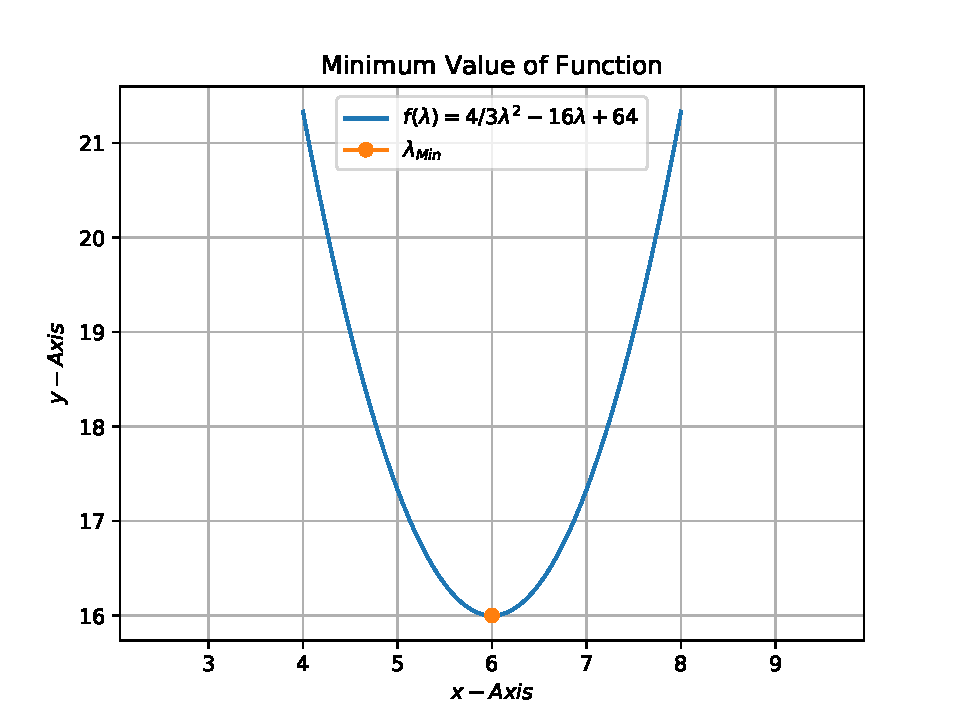
\includegraphics[width=\columnwidth]{figs/problem3.1a.pdf}
	\end{center}
\caption{}
\label{fig:Fig1}
\end{figure}
\begin{figure}[!h]
	\begin{center}
		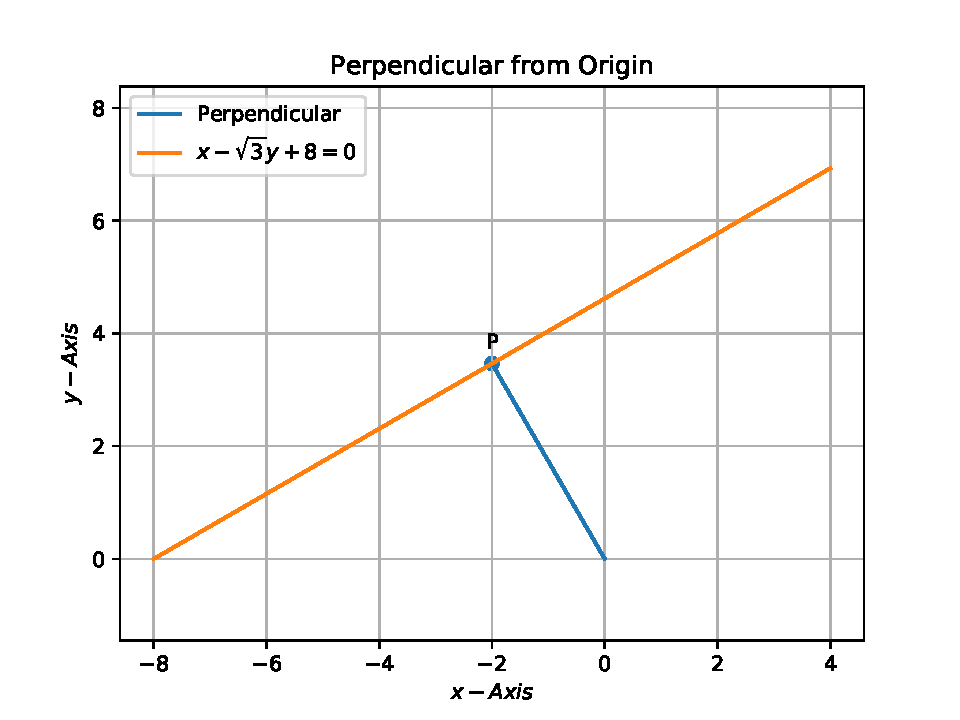
\includegraphics[width=\columnwidth]{figs/problem3.1b.pdf}
	\end{center}
\caption{}
\label{fig:Fig2}
\end{figure}
\end{enumerate}
\end{document}
